\section{Attitude reference}
For the satellite to be able to track a given static position on Earth within 1°, a quaternion is computed. Therefore, this quaternion represents the vector that points from the orbit position to the station.

The tracking quaternion is calculated by giving a quaternion attitude demand in orbit frame and by using this it is possible to calculate the angular velocity demand. The position vector of the station and the position of the satellite are known, then this two are subtracted and results the direction between them which is transformed into a quaternion.

In the simulation the Earth station is stationary which means that it does not move in the inertial frame.

The way it can be verify that the error is around 1°, is by looking at the attitude error quaternion.  The scalar part which represent $\cos (\frac{\alpha}{2}) $ and then calculate $\alpha$ based on that.  That $\alpha$ it should not be bigger then 1°.

\begin{figure}[H]
	\centering
	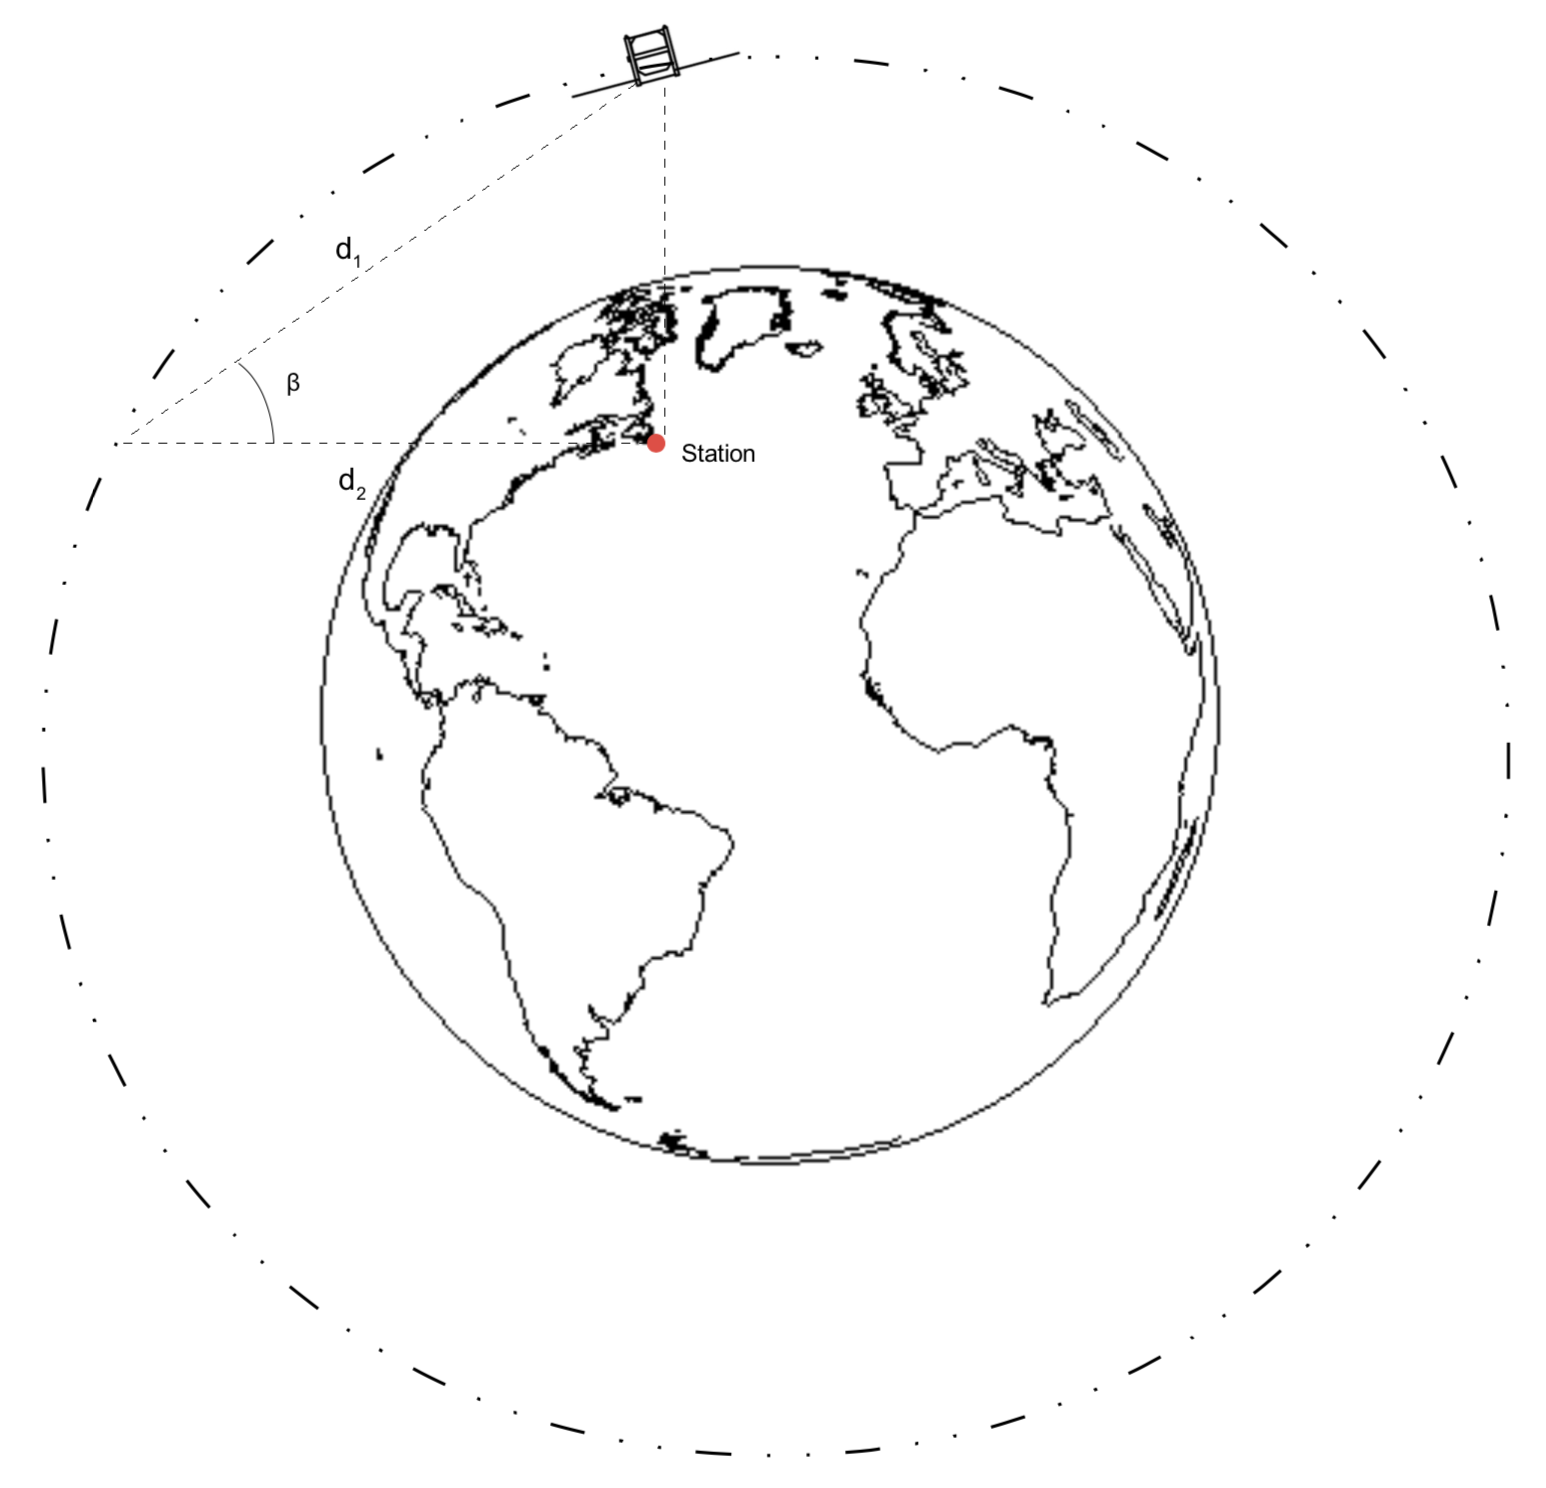
\includegraphics[width=0.6\linewidth]{figures/TS}
	\caption{Tracking a target on Earth }
	\label{fig:TS}
\end{figure}

 